\DailyTitle{6333 Log (October 27, 2010)}

\DailySection{Goals}

\begin{enumerate}
\item By the end of the day, have a working version of hcal tree and start running
\item Copy the toy MC code to desktop and start running
\end{enumerate}

\DailySection{Summary List}

\begin{enumerate}
\item Implemented the new hcal pulse tree that has MET information and also event cleaning variables.
\end{enumerate}

\DailySection{Number of pulses above threshold estimation}

Test run on DQM on express physics stream on a few recent runs.
The result is similar across runs, and one example is shown in figure \ref{Figure_6333NumberOfPulseAbove10fC}.
From the slope and number of events there, assuming it's an exponential drop, by the time we reach $10^6$ events,
the expected number of event line will cross the 1-event level at 190-200 counts.
Therefore setting the limit to 250-300 should be enough for our purpose.

\begin{figure}
   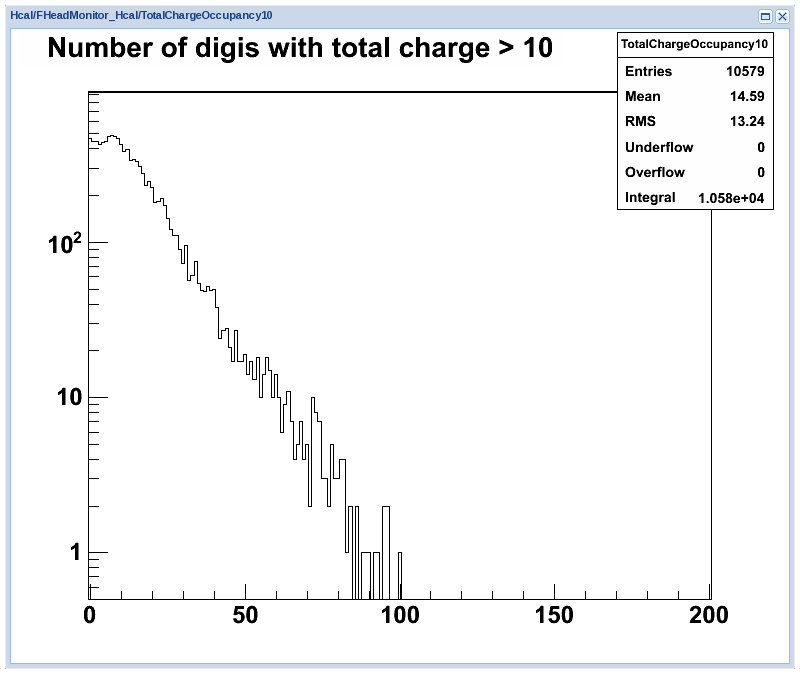
\includegraphics[width=120mm]{DailyLog/6333/6333NumberOfPulseAbove10fC.png}
   \caption{Estimation of upper limit for number of pulses in an event.}
   \label{Figure_6333NumberOfPulseAbove10fC}
\end{figure}

\DailySection{Implementing new Hcal pulse shape tree}

\DailySubSection{Specifications of the double-chi2 tree (6333 version)}

The new tree will include the following:

\begin{enumerate}
\item Event coordinate: event number, run number, lumi section, bunch crossing, orbit (?), time
\item All pulses above 10 fC: charges, pedestals, energy, ieta, iphi, depth
\item Calorimeter energies: ET vector, sum E, sum |ET| of HB, HE, HF, EE, EB.  We should be able to reconstruct MET from these later.
\item Also MET from the nominal calomet object.
\item Triggers: technical, L1, HLT
\item Event cleaning related: number of good tracks, total pt (both scalar and vector sum) of good tracks, number of good primary vertices.
\end{enumerate}

The ``good track'' is selected by these requirements:

\begin{enumerate}
\item PT within 0.5-500 GeV/c
\item $\chi^2/ndof < 20$
\item $|\eta| < 2.4$
\item Valid hit at least 6
\item No requirement on compatibility to PV, since this is going to be used as event selection, and no serious use of the tracks is intended.
\end{enumerate}

\DailySubSection{Time and space estimation of the tree}

Tried run on 200 events from the \texttt{RAW} \text{Jet} dataset (run 148058) interactively on lxplus.

Time usage is

\begin{verbatim}
real    11m18.164s
user    11m1.374s
sys     0m4.953s
\end{verbatim}

and the output root file has size of 745 kB.  So it is about 3.3 kB per event, and it takes on average 3.39 seconds every event.
The single root file I copied out from run 148058 (\texttt{Jet} dataset, \texttt{RAW}) has about 20000 events.  This translates to 67800 seconds, or 18 hours.
There should be plenty of time before next Thursday for them to run.  20000 events will have file size of roughly 73 MB.

Let's say we start the production on two/three runs, evaluate/debug what we need for one or two days, and rerun for real for more runs in preparation for Thursday update.

Started running on \texttt{Jet} dataset and \texttt{HcalHPDNoise} stream, run 147454, 147754 and 148058.  Expect roughly a day for all to finish.


\DailySection{Reflection}

\DailySection{Goals for next work day}

\begin{enumerate}
\item Eat lunch
\item Eat dinner
\item Find the red herring
\end{enumerate}


